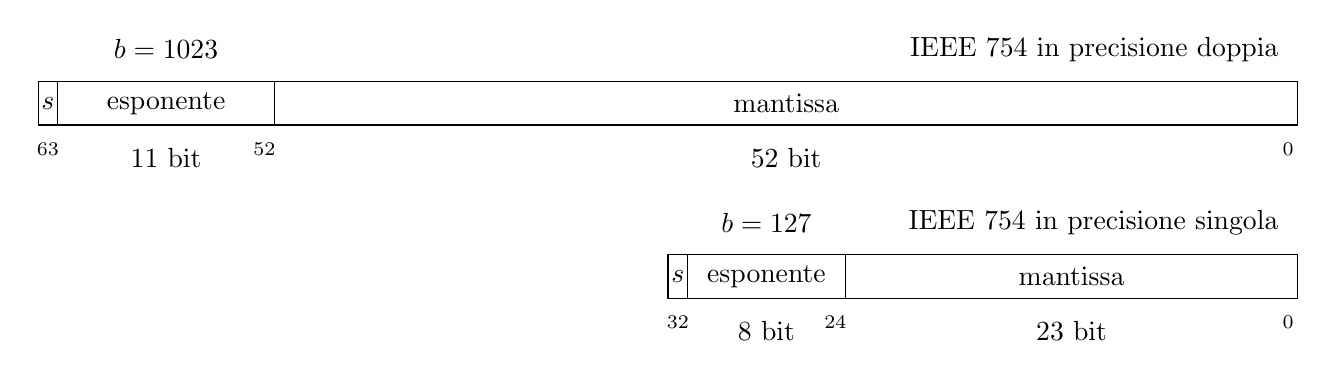
\begin{tikzpicture}[main node/.style={rectangle,draw, inner sep=0.,outer sep=0.}]%
  \pgfmathsetmacro{\xscale}{0.25}
  \pgfmathsetmacro{\yscale}{0.55}
  \draw[draw=black] (0., 0.) rectangle (1. * \xscale, 1. * \yscale);
  \draw[draw=black] (1. * \xscale, 0.) rectangle (12. * \xscale, 1. * \yscale);
  \draw[draw=black] (12. * \xscale, 0.) rectangle (64. * \xscale, 1. * \yscale);
  \node at (0.5 * \xscale, 0.5 * \yscale) {$s$};
  \node at (0.5 * \xscale, -0.55 * \yscale) {\scriptsize{$63$}};
  \node at (11.5 * \xscale, -0.55 * \yscale) {\scriptsize{$52$}};
  \node at (63.5 * \xscale, -0.55 * \yscale) {\scriptsize{$0$}};
  \node at (6.5 * \xscale, 0.5 * \yscale) {esponente};
  \node at (38. * \xscale, 0.5 * \yscale) {mantissa};
  \node[anchor=east] at (63.5 * \xscale, 1.75 * \yscale) {IEEE 754 in precisione doppia};
  \node at (6.5 * \xscale, 1.75 * \yscale) {$b=1023$};
  \node at (6.5 * \xscale, -0.75 * \yscale) {$11$~bit};
  \node at (38. * \xscale, -0.75 * \yscale) {$52$~bit};

  \draw[draw=black] (32. * \xscale, -4. * \yscale) rectangle (33. * \xscale, -3. * \yscale);
  \draw[draw=black] (33. * \xscale, -4. * \yscale) rectangle (41. * \xscale, -3. * \yscale);
  \draw[draw=black] (41. * \xscale, -4. * \yscale) rectangle (64. * \xscale, -3. * \yscale);
  \node at (32.5 * \xscale, -3.5 * \yscale) {$s$};
  \node at (32.5 * \xscale, -4.55 * \yscale) {\scriptsize{$32$}};
  \node at (40.5 * \xscale, -4.55 * \yscale) {\scriptsize{$24$}};
  \node at (63.5 * \xscale, -4.55 * \yscale) {\scriptsize{$0$}};
  \node at (37.0 * \xscale, -3.5 * \yscale) {esponente};
  \node at (52.5 * \xscale, -3.5 * \yscale) {mantissa};
  \node[anchor=east] at (63.5 * \xscale, -2.25 * \yscale) {IEEE 754 in precisione singola};
  \node at (37.0 * \xscale, -2.25 * \yscale) {$b=127$};
  \node at (37. * \xscale, -4.75 * \yscale) {$8$~bit};
  \node at (52.5 * \xscale, -4.75 * \yscale) {$23$~bit};

\end{tikzpicture}
